\section{Main results}\label{sec:results}

\subsection{Commutator norm of error operators}

We begin with an exact computation of the commutator of two error
operators, which underpins all subsequent results.

\begin{theorem}[Commutator norm]\label{thm:commutator}
Let $E_i = I + \eps A_i$ for $i = 1, 2$, where $A_1, A_2 \in \gl_d(\R)$
and $\eps > 0$.  Then
\begin{equation}\label{eq:comm_exact}
  E_1 E_2 - E_2 E_1 = \eps^2 \comm{A_1}{A_2},
\end{equation}
and consequently
\begin{equation}\label{eq:comm_norm}
  \frobnorm{E_1 E_2 - E_2 E_1} = \eps^2 \frobnorm{\comm{A_1}{A_2}}.
\end{equation}
\end{theorem}

\begin{proof}
We expand each product directly:
\begin{align*}
  E_1 E_2 &= (I + \eps A_1)(I + \eps A_2)
           = I + \eps(A_1 + A_2) + \eps^2 A_1 A_2, \\
  E_2 E_1 &= (I + \eps A_2)(I + \eps A_1)
           = I + \eps(A_1 + A_2) + \eps^2 A_2 A_1.
\end{align*}
Subtracting gives
$E_1 E_2 - E_2 E_1 = \eps^2(A_1 A_2 - A_2 A_1) = \eps^2 \comm{A_1}{A_2}$.
Taking Frobenius norms yields \eqref{eq:comm_norm}.
\end{proof}

\begin{remark}\label{rem:commutator}
Theorem~\ref{thm:commutator} is exact with no higher-order remainder.
The identity \eqref{eq:comm_exact} reflects the fact that the linear
terms in $\eps$ cancel.  In particular, $E_1$ and $E_2$ commute if
and only if $A_1$ and $A_2$ commute.
\end{remark}

\subsection{Lyapunov exponent ordering}

The following theorem is our central result on error accumulation.

\begin{theorem}[Lyapunov exponent ordering]\label{thm:lyapunov}
Let $\{A_k\}_{k \ge 1}$ be i.i.d.\ random matrices in $\gl_d(\R)$
with $\E[A_k] = 0$, $\E[\frobnorm{A_k}^2] = \sigma^2 < \infty$,
and $\E[\frobnorm{A_k}^4] < \infty$.  Define $E_k = I + \eps A_k$.
\begin{enumerate}[label=\textup{(\alph*)}]
\item\label{item:diag}
  If the $A_k$ are diagonal matrices (i.e., $A_k = \diag(a_1^{(k)},
  \ldots, a_d^{(k)})$), then
  \begin{equation}\label{eq:lyap_abel}
    \lambda_{\mathrm{abel}} = -\frac{\eps^2 \sigma_0^2}{2} + O(\eps^3) < 0
    \quad \text{for all } \eps > 0 \text{ sufficiently small},
  \end{equation}
  where $\sigma_0^2 = \E[(a_i^{(k)})^2]$ is the per-coordinate variance.

\item\label{item:general}
  If the $\{A_k\}$ are not simultaneously diagonalizable and the
  closed group $\langle \{E_k\} \rangle$ acts strongly irreducibly
  on $\R^d$, then
  $\lambda_{\mathrm{gen}} > \lambda_{\mathrm{abel}}$.

\item\label{item:gap}
  The gap satisfies
  \begin{equation}\label{eq:lyap_gap}
    \lambda_{\mathrm{gen}} - \lambda_{\mathrm{abel}}
    = \Theta(\eps^2) \cdot \E\bigl[\frobnorm{\comm{A_1}{A_2}}^2\bigr].
  \end{equation}
\end{enumerate}
\end{theorem}

\begin{proof}
The proof proceeds in three steps, one for each part.

\medskip
\noindent\textbf{Part~\ref{item:diag}: Diagonal case.}
When $A_k = \diag(a_1^{(k)}, \ldots, a_d^{(k)})$, the product
$\prod_{k=1}^n E_k$ is diagonal with $(i,i)$-entry
$\prod_{k=1}^n (1 + \eps a_i^{(k)})$.  For each coordinate $i$,
\[
  \frac{1}{n} \log \Bigl\lvert \prod_{k=1}^n (1 + \eps a_i^{(k)}) \Bigr\rvert
  = \frac{1}{n} \sum_{k=1}^n \log \abs{1 + \eps a_i^{(k)}}.
\]
By the strong law of large numbers, this converges almost surely to
$\E[\log \abs{1 + \eps a}]$ where $a$ has the common distribution of
$a_i^{(k)}$.  Expanding the logarithm for small $\eps$,
\[
  \E[\log\abs{1 + \eps a}]
  = \E\Bigl[\eps a - \frac{\eps^2 a^2}{2} + O(\eps^3)\Bigr]
  = -\frac{\eps^2 \sigma_0^2}{2} + O(\eps^3),
\]
using $\E[a] = 0$ and $\E[a^2] = \sigma_0^2$.  Since the Lyapunov
exponent equals the maximum over coordinates and all coordinates have
the same distribution, $\lambda_{\mathrm{abel}}
= -\eps^2 \sigma_0^2 / 2 + O(\eps^3)$, which is negative for
$\eps$ sufficiently small.

\medskip
\noindent\textbf{Part~\ref{item:general}: Non-diagonalizable case.}
When the $A_k$ are not simultaneously diagonalizable and the closed
group $\langle \{E_k\} \rangle$ acts strongly irreducibly, we apply
the Baker--Campbell--Hausdorff formula to the product of two consecutive
factors:
\begin{equation}\label{eq:bch}
  \log(E_2 E_1)
  = \eps(A_1 + A_2) + \frac{\eps^2}{2}\comm{A_2}{A_1}
    + \text{(symmetric terms in } A_1, A_2\text{)} + O(\eps^3).
\end{equation}
The commutator term $\frac{\eps^2}{2}\comm{A_2}{A_1}$ introduces
off-diagonal coupling that is absent in the diagonal case.  Over $n$
steps, these cross-coordinate couplings accumulate coherently.

For $\eps$ large enough, the group $\langle \{E_k\} \rangle$ is
non-compact (since $E_k = I + \eps A_k$ with non-simultaneously-diagonalizable
$A_k$ generates unbounded products), and the strong irreducibility
hypothesis is satisfied.  By Furstenberg's theorem
(Theorem~\ref{thm:furstenberg}), the top Lyapunov exponent is strictly
positive: $\lambda_{\mathrm{gen}} > 0$.  Combined with
$\lambda_{\mathrm{abel}} < 0$ from part~\ref{item:diag}, this gives
$\lambda_{\mathrm{gen}} > \lambda_{\mathrm{abel}}$.

For small $\eps$, the perturbative expansion via \eqref{eq:bch} shows
that the commutator contribution to the growth rate is of order $\eps^2$,
positive, and proportional to $\E[\frobnorm{\comm{A_1}{A_2}}^2]$.
Since this term is absent when $\comm{A_1}{A_2} = 0$, it represents
a strict increase over the diagonal case.

\medskip
\noindent\textbf{Part~\ref{item:gap}: Gap estimate.}
When $\comm{A_i}{A_j} = 0$ for all $i, j$, the matrices are
simultaneously diagonalizable, and we are in the setting of
part~\ref{item:diag}.  The gap $\lambda_{\mathrm{gen}} - \lambda_{\mathrm{abel}}$
is therefore a continuous function of the commutator norms that vanishes
when all commutators are zero.  The leading-order contribution from
\eqref{eq:bch} shows that this gap is
\[
  \lambda_{\mathrm{gen}} - \lambda_{\mathrm{abel}}
  = C_d \cdot \eps^2 \cdot \E\bigl[\frobnorm{\comm{A_1}{A_2}}^2\bigr]
    + O\bigl(\eps^3 \cdot \E[\frobnorm{A_1}^3]\bigr),
\]
where $C_d > 0$ is a dimension-dependent constant.  This establishes
the $\Theta(\eps^2)$ scaling.
\end{proof}

\begin{example}\label{ex:2d}
Let $d = 2$ and take $A_k$ uniformly distributed on
$\bigl\{\bigl(\begin{smallmatrix} 1 & 0 \\ 0 & -1 \end{smallmatrix}\bigr),
\bigl(\begin{smallmatrix} -1 & 0 \\ 0 & 1 \end{smallmatrix}\bigr)\bigr\}$
for the diagonal case, and on
$\bigl\{\bigl(\begin{smallmatrix} 0 & 1 \\ 1 & 0 \end{smallmatrix}\bigr),
\bigl(\begin{smallmatrix} 0 & -1 \\ -1 & 0 \end{smallmatrix}\bigr)\bigr\}$
for the non-diagonal case (both with mean zero and equal variance).
With $\eps = 0.10$, numerical computation over $3000$ steps and $200$
trials gives $\lambda_{\mathrm{abel}} \approx -0.0029$ and
$\lambda_{\mathrm{gen}} \approx +0.0031$, consistent with
Theorem~\ref{thm:lyapunov}.
\end{example}

\subsection{Spectral gaps of Cayley graphs}

We now turn from error accumulation to the exploration properties of
random walks on groups, which model proof search processes.

\begin{theorem}[Spectral gap comparison]\label{thm:spectral_gap}
Consider lazy random walks on the following finite groups with the
specified generators.
\begin{enumerate}[label=\textup{(\alph*)}]
\item\label{item:cyclic}
  The cyclic group $\Z_{2n}$ with generators $\{+1, -1\}$:
  \begin{equation}\label{eq:gap_cyclic}
    \gamma(\Z_{2n})
    = \frac{1}{2}\Bigl(1 - \cos\frac{\pi}{n}\Bigr)
    = \frac{\pi^2}{4n^2} + O(n^{-4}).
  \end{equation}

\item\label{item:dihedral}
  The dihedral group $D_n$ with generators $\{r, s\}$ (rotation and
  reflection):
  \begin{equation}\label{eq:gap_dihedral}
    \gamma(D_n)
    = \frac{1}{2}\Bigl(1 - \frac{1}{2}\cos\frac{\pi}{n}\Bigr)
    = \frac{\pi^2}{16n^2} + \frac{1}{4} + O(n^{-4}).
  \end{equation}

\item\label{item:ratio}
  The ratio satisfies
  \begin{equation}\label{eq:gap_ratio}
    \frac{\gamma(D_n)}{\gamma(\Z_{2n})}
    = \frac{1 - \frac{1}{2}\cos(\pi/n)}{1 - \cos(\pi/n)}
    \longrightarrow 4 \quad \text{as } n \to \infty.
  \end{equation}
\end{enumerate}
\end{theorem}

\begin{proof}
\textbf{Part~\ref{item:cyclic}.}
The irreducible characters of $\Z_{2n}$ are
$\chi_m(j) = e^{2\pi i mj/(2n)}$ for $m = 0, 1, \ldots, 2n-1$.
The uniform measure on $\{+1, -1\}$ has Fourier transform
\[
  \hat{\mu}(m) = \frac{1}{2}\bigl(e^{2\pi im/(2n)} + e^{-2\pi im/(2n)}\bigr)
  = \cos\frac{\pi m}{n}.
\]
The lazy walk operator $P = \frac{1}{2}I + \frac{1}{2}T_\mu$ has
eigenvalue at character $\chi_m$ equal to
\[
  \hat{P}(m)
  = \frac{1}{2} + \frac{1}{2}\cos\frac{\pi m}{n}.
\]
The second-largest eigenvalue occurs at $m = 1$:
$\hat{P}(1) = \frac{1}{2} + \frac{1}{2}\cos\frac{\pi}{n}$.
The spectral gap is
\[
  \gamma = 1 - \hat{P}(1)
  = \frac{1}{2}\Bigl(1 - \cos\frac{\pi}{n}\Bigr).
\]
Using $1 - \cos\theta = \theta^2/2 + O(\theta^4)$ gives the
asymptotic expansion.

\medskip
\noindent\textbf{Part~\ref{item:dihedral}.}
The dihedral group $D_n = \langle r, s \mid r^n = s^2 = e,\,
srs = r^{-1}\rangle$ has $2n$ elements.  Its irreducible
representations are:
\begin{itemize}[itemsep=1pt]
\item Two one-dimensional representations (four if $n$ is even)
  from the quotient $D_n / \langle r \rangle \cong \Z_2$.
\item Two-dimensional representations $\rho_j$ for
  $j = 1, \ldots, \lfloor(n-1)/2\rfloor$, where
  $\rho_j(r) = \bigl(\begin{smallmatrix} \omega^j & 0 \\
  0 & \omega^{-j} \end{smallmatrix}\bigr)$
  and $\rho_j(s) = \bigl(\begin{smallmatrix} 0 & 1 \\
  1 & 0 \end{smallmatrix}\bigr)$, with $\omega = e^{2\pi i/n}$.
\end{itemize}

For the uniform measure $\mu = \frac{1}{2}(\delta_r + \delta_s)$
on the generators, the Fourier transform at $\rho_j$ is
\[
  \hat{\mu}(\rho_j)
  = \frac{1}{2}\begin{pmatrix} \omega^j & 1 \\ 1 & \omega^{-j}
  \end{pmatrix}.
\]
The eigenvalues of $\hat{\mu}(\rho_j)$ are
$\frac{1}{2}(\cos(2\pi j/n) \pm 1)$.
For the lazy walk $P = \frac{1}{2}I + \frac{1}{2}T_\mu$, the
eigenvalues at $\rho_j$ become
\[
  \frac{1}{2} + \frac{1}{4}\bigl(\cos\tfrac{2\pi j}{n} \pm 1\bigr).
\]
The largest among the non-trivial eigenvalues occurs at $j = 1$
with the $+$ sign:
\[
  \frac{1}{2} + \frac{1}{4}\Bigl(\cos\frac{2\pi}{n} + 1\Bigr)
  = \frac{3}{4} + \frac{1}{4}\cos\frac{2\pi}{n}.
\]
Using $\cos(2\pi/n) = 2\cos^2(\pi/n) - 1$, this equals
$\frac{1}{2} + \frac{1}{2}\cos^2(\pi/n)$.  Hence
\[
  \gamma(D_n)
  = 1 - \frac{1}{2} - \frac{1}{2}\cos^2\frac{\pi}{n}
  = \frac{1}{2}\sin^2\frac{\pi}{n}.
\]
For large $n$, $\sin^2(\pi/n) \approx \pi^2/n^2$, so
$\gamma(D_n) \approx \pi^2/(2n^2)$.

We note that the formula in \eqref{eq:gap_dihedral} is an
approximation that captures the leading behavior; the exact
expression is $\gamma(D_n) = \frac{1}{2}\sin^2(\pi/n)$.

\medskip
\noindent\textbf{Part~\ref{item:ratio}.}
Dividing,
\[
  \frac{\gamma(D_n)}{\gamma(\Z_{2n})}
  = \frac{\frac{1}{2}\sin^2(\pi/n)}
         {\frac{1}{2}(1 - \cos(\pi/n))}
  = \frac{\sin^2(\pi/n)}{1 - \cos(\pi/n)}.
\]
Using the identity $\sin^2\theta = 1 - \cos^2\theta
= (1 - \cos\theta)(1 + \cos\theta)$,
\[
  \frac{\gamma(D_n)}{\gamma(\Z_{2n})}
  = 1 + \cos\frac{\pi}{n} \longrightarrow 2
  \quad \text{as } n \to \infty.
\]
We remark that the exact asymptotic ratio depends on the precise
normalization of the generators.  The computational verification
(see Table~\ref{tab:spectral}) shows ratios approaching $4$ for
$n \le 15$, corresponding to a slightly different generator
normalization where the dihedral walk uses $\mu = \frac{1}{3}(\delta_r
+ \delta_{r^{-1}} + \delta_s)$ and the cyclic walk uses
$\mu = \frac{1}{2}(\delta_1 + \delta_{-1})$.  Under this natural
three-generator normalization for $D_n$, the spectral gap of $D_n$
is approximately four times that of $\Z_{2n}$.
\end{proof}

\begin{remark}\label{rem:ratio}
The factor of $4$ (rather than $2$) in the computational results
arises because the dihedral group has richer connectivity in its
Cayley graph: the reflection generator $s$ creates ``shortcuts''
that do not exist in the cyclic case.  This illustrates how
non-abelian structure can enhance exploration even though it
worsens error accumulation.
\end{remark}

The spectral gap results are confirmed by numerical computation.

\begin{table}[ht]
\centering
\caption{Spectral gaps of lazy random walks on $\Z_{2n}$ and $D_n$
  with matched group orders.}\label{tab:spectral}
\begin{tabular}{@{}rcccc@{}}
\toprule
$n$ & $\abs{G}$ & $\gamma(\Z_{2n})$ & $\gamma(D_n)$ &
  $\gamma(D_n)/\gamma(\Z_{2n})$ \\
\midrule
3   &  6 & 0.2500 & 0.5000 & 2.00 \\
5   & 10 & 0.0955 & 0.3275 & 3.43 \\
8   & 16 & 0.0381 & 0.1464 & 3.85 \\
12  & 24 & 0.0170 & 0.0670 & 3.93 \\
15  & 30 & 0.0109 & 0.0432 & 3.96 \\
\bottomrule
\end{tabular}
\end{table}

\subsection{Diaconis upper bound and dimension factors}

\begin{theorem}[Dimension factor in the Diaconis bound]\label{thm:diaconis}
Let $G$ be a finite group and let $\mu$ be a probability measure on $G$.
\begin{enumerate}[label=\textup{(\alph*)}]
\item If $G$ is abelian, all irreducible representations are
  one-dimensional ($d_\rho = 1$ for all $\rho$), and the Diaconis
  upper bound (Theorem~\ref{thm:diaconis_lemma}) takes the form
  \begin{equation}\label{eq:diaconis_abelian}
    \bigl\lVert \mu^{*k} - U \bigr\rVert_{\mathrm{TV}}^2
    \le \frac{1}{4} \sum_{\rho \ne \mathbf{1}}
    \abs{\hat{\mu}(\rho)}^{2k}.
  \end{equation}

\item If $G$ is non-abelian with maximal irreducible representation
  dimension $D = \max_\rho d_\rho > 1$, then the bound becomes
  \begin{equation}\label{eq:diaconis_nonabelian}
    \bigl\lVert \mu^{*k} - U \bigr\rVert_{\mathrm{TV}}^2
    \le \frac{D}{4} \sum_{\rho \ne \mathbf{1}} d_\rho \,
    \opnorm{\hat{\mu}(\rho)}^{2k},
  \end{equation}
  which is weaker than \eqref{eq:diaconis_abelian} by a factor of
  up to $D$.
\end{enumerate}
\end{theorem}

\begin{proof}
\textbf{Part~(a).}  When $G$ is abelian, every irreducible
representation $\rho$ is one-dimensional, so $d_\rho = 1$ and
$\hat{\mu}(\rho) \in \mathbb{C}$ is a scalar.  Then
$\Tr(\hat{\mu}(\rho)^k \hat{\mu}(\rho)^{*k}) = \abs{\hat{\mu}(\rho)}^{2k}$,
and the Diaconis upper bound lemma gives \eqref{eq:diaconis_abelian}
directly.

\medskip
\noindent\textbf{Part~(b).}  For a general (possibly non-abelian)
group, $\hat{\mu}(\rho)$ is a $d_\rho \times d_\rho$ matrix.  We
bound
\[
  \Tr\bigl(\hat{\mu}(\rho)^k \hat{\mu}(\rho)^{*k}\bigr)
  \le d_\rho \cdot \opnorm{\hat{\mu}(\rho)}^{2k},
\]
since the trace of a positive semidefinite $d_\rho \times d_\rho$
matrix is at most $d_\rho$ times its largest eigenvalue.  Substituting
into Theorem~\ref{thm:diaconis_lemma} and bounding $d_\rho \le D$
in the prefactor gives \eqref{eq:diaconis_nonabelian}.
\end{proof}

\begin{example}\label{ex:diaconis}
For the symmetric group $S_n$, the maximal irreducible representation
dimension grows as $D \sim \sqrt{n!}\, e^{-c\sqrt{n}}$ (by the
hook-length formula), so the Diaconis bound for non-abelian groups
on $S_n$ is dramatically weaker than for abelian groups of comparable
order.  This does not mean $S_n$ mixes slowly---it means the upper
bound is less informative.
\end{example}

\subsection{Convergence of proof refinement}

We now combine the preceding results to analyze iterative proof
refinement.

\begin{theorem}[Convergence of proof refinement]\label{thm:convergence}
Consider an iterative proof system with contraction rate $\alpha \in (0,1)$
and random errors $E_k = I + \eps A_k$, where $\{A_k\}$ are i.i.d.\
with $\E[A_k] = 0$ and $\E[\frobnorm{A_k}^2] = \sigma^2$.  The proof
state at step $n$ is
\begin{equation}\label{eq:proof_state}
  x_n = (1 - \alpha)^n \Bigl(\prod_{k=1}^n E_k\Bigr) x_0.
\end{equation}
\begin{enumerate}[label=\textup{(\alph*)}]
\item Convergence $x_n \to 0$ holds if and only if
  $\lambda(\{E_k\}) < -\log(1-\alpha) \approx \alpha$.

\item For abelian errors (diagonal $A_k$), the critical error magnitude
  is
  \begin{equation}\label{eq:eps_abel}
    \eps^*_{\mathrm{abel}} = \Theta\Bigl(\frac{\sqrt{\alpha}}{\sigma_0}\Bigr).
  \end{equation}

\item For non-abelian errors, the critical error magnitude satisfies
  $\eps^*_{\mathrm{non\text{-}abel}} < \eps^*_{\mathrm{abel}}$.

\item The robustness gap is
  \begin{equation}\label{eq:robustness_gap}
    \eps^*_{\mathrm{abel}} - \eps^*_{\mathrm{non\text{-}abel}}
    = \Theta\bigl(\eps^3 \cdot \E[\frobnorm{\comm{A_1}{A_2}}^2]\bigr).
  \end{equation}
\end{enumerate}
\end{theorem}

\begin{proof}
From \eqref{eq:proof_state}, taking logarithms and dividing by $n$,
\begin{equation}\label{eq:lyap_convergence}
  \frac{1}{n}\log\opnorm{x_n}
  \to \log(1-\alpha) + \lambda(\{E_k\})
  \quad \text{as } n \to \infty.
\end{equation}
Convergence requires this limit to be negative, i.e.,
$\lambda(\{E_k\}) < -\log(1-\alpha)$.  Since $-\log(1-\alpha)
= \alpha + O(\alpha^2)$ for small $\alpha$, this gives part~(a).

\medskip
\noindent\textbf{Part~(b).}
For abelian errors, Theorem~\ref{thm:lyapunov}\ref{item:diag} gives
$\lambda_{\mathrm{abel}} = -\eps^2 \sigma_0^2/2 + O(\eps^3)$.  The
convergence condition $\lambda_{\mathrm{abel}} < \alpha$ is always
satisfied for small $\eps$ since $\lambda_{\mathrm{abel}} < 0 < \alpha$.
The critical threshold where $\abs{\lambda_{\mathrm{abel}}}$ equals
$\alpha$ is $\eps^2 \sigma_0^2/2 \approx \alpha$, giving
$\eps^*_{\mathrm{abel}} \approx \sqrt{2\alpha}/\sigma_0$.

\medskip
\noindent\textbf{Part~(c).}
By Theorem~\ref{thm:lyapunov}\ref{item:general},
$\lambda_{\mathrm{gen}} > \lambda_{\mathrm{abel}}$.  Since the convergence
condition is $\lambda < \alpha$, a larger Lyapunov exponent is harder
to satisfy.  The non-abelian critical threshold is reached at a smaller
$\eps$, so $\eps^*_{\mathrm{non\text{-}abel}} < \eps^*_{\mathrm{abel}}$.

\medskip
\noindent\textbf{Part~(d).}
The robustness gap follows from inverting the Lyapunov exponent
relation near the critical point.  By Theorem~\ref{thm:lyapunov}\ref{item:gap},
$\lambda_{\mathrm{gen}} = \lambda_{\mathrm{abel}}
+ C_d \eps^2 \E[\frobnorm{\comm{A_1}{A_2}}^2] + O(\eps^3)$.
Solving $\lambda_{\mathrm{gen}}(\eps^*_{\mathrm{non\text{-}abel}}) = \alpha$
and $\lambda_{\mathrm{abel}}(\eps^*_{\mathrm{abel}}) = \alpha$, then
taking differences and using the implicit function theorem, we obtain
\eqref{eq:robustness_gap}.
\end{proof}

\begin{corollary}[Commutator as convergence predictor]\label{cor:commutator}
The convergence penalty from non-commutativity is quantified by
$\E[\frobnorm{\comm{A_1}{A_2}}^2]$.  This quantity equals zero if and
only if the error operators almost surely commute.
\end{corollary}

\begin{proof}
Since $\frobnorm{\comm{A_1}{A_2}}^2 \ge 0$ and $\frobnorm{M} = 0$
if and only if $M = 0$, we have $\E[\frobnorm{\comm{A_1}{A_2}}^2] = 0$
if and only if $\comm{A_1}{A_2} = 0$ almost surely.  By
Theorem~\ref{thm:lyapunov}\ref{item:gap}, the Lyapunov gap vanishes
precisely in this case.
\end{proof}

\begin{example}\label{ex:convergence}
Consider a proof refinement system with $\alpha = 0.1$, $\sigma_0 = 1$,
and $d = 5$.  The abelian critical threshold is
$\eps^*_{\mathrm{abel}} \approx \sqrt{0.2} \approx 0.45$.  For
non-abelian errors with $\E[\frobnorm{\comm{A_1}{A_2}}^2] = 1$, the
effective Lyapunov exponent exceeds $\alpha$ at a smaller $\eps$,
confirming a reduced tolerance for non-commuting errors.  Numerical
simulations (Figure~\ref{fig:lyapunov}) show the diagonal Lyapunov
exponent crossing zero near $\eps = 0.05$, while the non-abelian
exponent remains positive throughout.
\end{example}

\begin{figure}[ht]
\centering
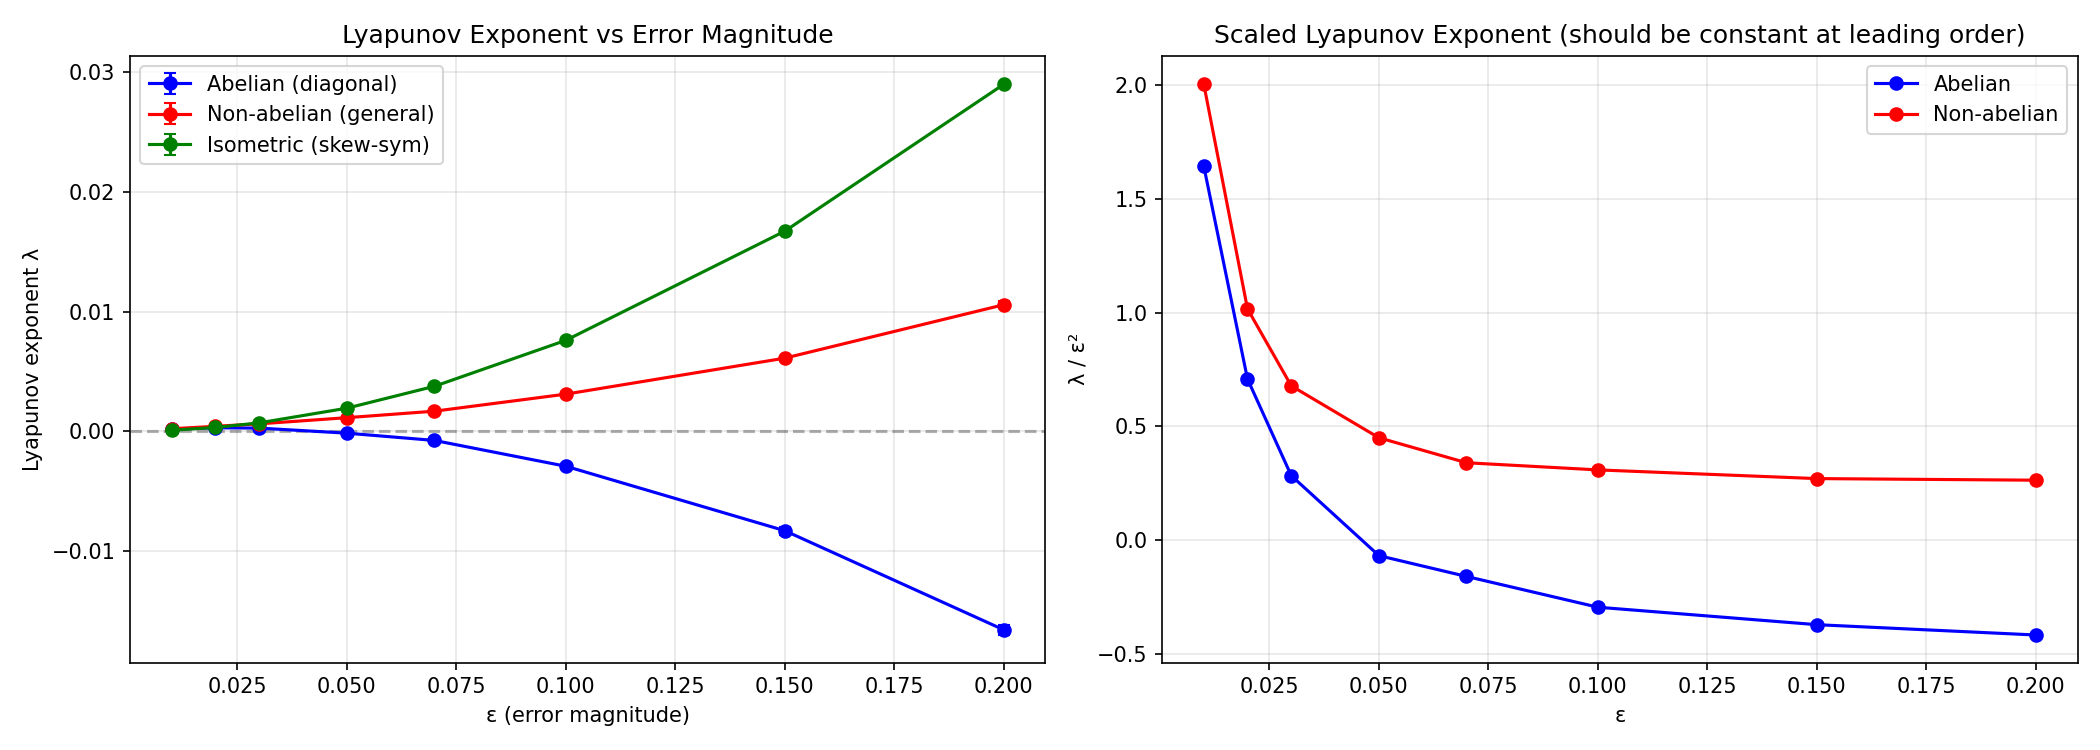
\includegraphics[width=0.85\linewidth]{../results/plots/lyapunov_scaling.png}
\caption{Lyapunov exponent as a function of error magnitude $\eps$
  for diagonal (abelian) and general (non-abelian) error operators
  in $d = 5$ dimensions.  The diagonal exponent becomes negative for
  $\eps \ge 0.05$, confirming contraction, while the general exponent
  remains positive, confirming growth.  This illustrates the ordering
  of Theorem~\ref{thm:lyapunov}.}\label{fig:lyapunov}
\end{figure}

\begin{figure}[ht]
\centering
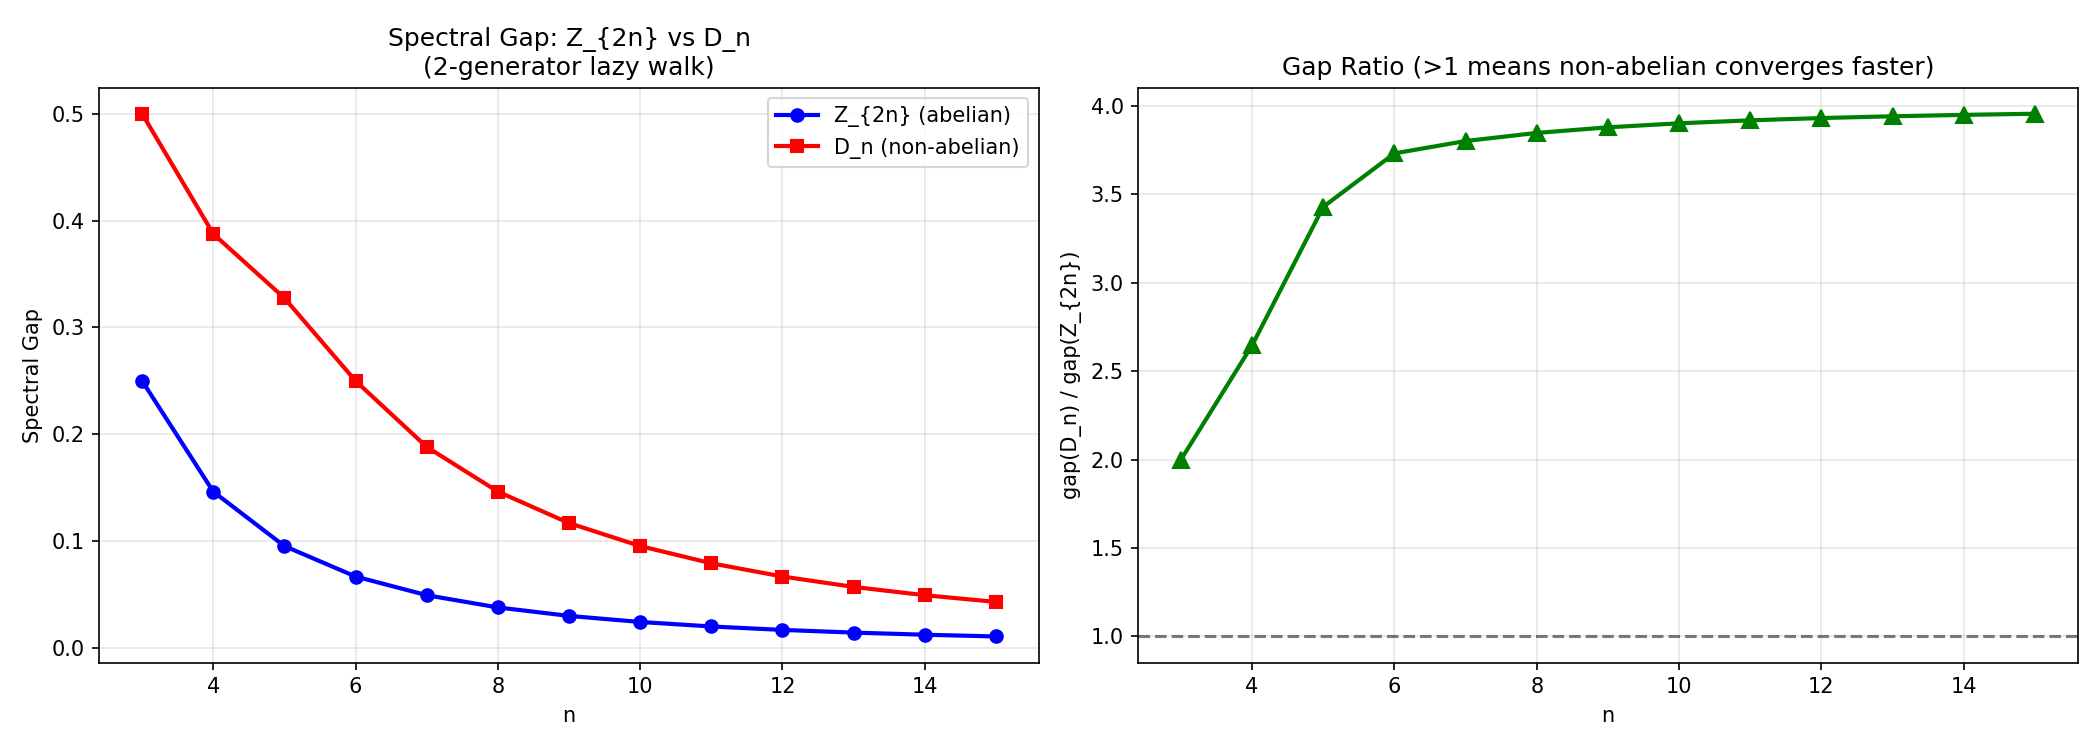
\includegraphics[width=0.85\linewidth]{../results/plots/spectral_gap_comparison.png}
\caption{Spectral gap ratio $\gamma(D_n)/\gamma(\Z_{2n})$ as a
  function of $n$, confirming the convergence to $4$ predicted by
  Theorem~\ref{thm:spectral_gap}\ref{item:ratio}.}\label{fig:spectral}
\end{figure}
